% ==========================================================
\section{Behavioral Programming}
\label{sec:bp}
% ==========================================================

\gls{bp} is a paradigm for programming reactive systems~\cite{harel_behavioral_2012}.
It bridges the gap between requirements and implementation by expressing system behavior as executable scenarios and use cases.
\gls{bp} is based on independent scenarios that correspond to individual system requirements.
Given that each scenario acts as a standalone module, developers can incrementally extend and refine the system by adding new behaviors, rules, or tactics without changing existing code.
This development style makes \gls{bp} well-suited for complex, reactive systems~\cite{elyasaf_context-oriented_2021}.

% ----------------------------------------------------------
\subsection{Foundations of Behavioral Programming}
\label{subsec:bp_foundation}
% ----------------------------------------------------------

The primary building blocks of \gls{bp} are behavioral threads (b-threads)~\cite{harel_behavioral_2012}.
Each b-thread runs concurrently and captures one specific scenario that the system should or should not follow.
The b-threads are decoupled and typically do not know of one another.

B-threads communicate through an enhanced publish/subscribe protocol using the \texttt{bSync} method~\cite{harel_behavioral_2012}.
When a b-thread reaches a synchronization point, it invokes \texttt{bSync} and suspends execution until the arbiter evaluates the joint state of all b-threads.
At each synchronization point, every b-thread submits three sets of events to the event arbiter:
\begin{itemize}
\item \textbf{requested:} The b-thread proposes these events for execution and asks to be notified if they occur.
\item \textbf{waited-for:} These events are not triggered by the b-thread, but it asks to be notified if another thread successfully requests them.
\item \textbf{blocked:} The b-thread explicitly forbids these events from occurring, acting as a veto against other b-threads' requests.
\end{itemize}
An event is triggered only if at least one b-thread requests it and none block it~\cite{elyasaf_context-oriented_2021}.

% ----------------------------------------------------------
\subsection{Context-Oriented Behavioral Programming}
\label{subsec:bp_context-oriented}
% ----------------------------------------------------------

\gls{cobp}, formalized by Elyasaf~\cite{elyasaf_context-oriented_2021}, extends \gls{bp} by integrating dynamic environmental data and system state into the behavioral model.
In Harel's original \gls{bp}, systems are built from independent b-threads that communicate only by requesting, waiting for, and blocking events at synchronization points~\cite{harel_behavioral_2012}.
While this keeps threads isolated, it leaves no explicit, first-class mechanism for representing or changing context. 
As a result, sharing contextual data among b-threads requires structural workarounds~\cite{elyasaf_context-oriented_2021}.

Elyasaf addresses this in \gls{cobp} by introducing formal extensions to manage context natively.
Instead of standard b-threads, \gls{cobp} uses Context-Aware Behavioral Threads (CBTs), each bound to a query over the system's contextual data~\cite{elyasaf_context-oriented_2021}.
When a CBT's query yields a new result, the system spawns a live copy of that CBT, passing the query result as a local variable called the seed, allowing the thread to execute its logic in that specific context.
\gls{cobp} also connects behavioral events to data updates through an effect function, which translates selected events into updates to the contextual data structure before propagating the updated context to all live copies.

An empirical study suggests that this explicit context modeling helps developers comprehend complex, context-dependent guard rules~\cite{ashrov_study_2025}.
It is also well-suited for scalable systems that must adapt to changing conditions, such as smart devices and robotic controllers.
At the same time, \gls{cobp} introduces a steeper learning curve and higher cognitive load, which can make systems more difficult to comprehend and align with requirements than classical \gls{bp} does.

% ----------------------------------------------------------
\subsection{Water Tank Example}
\label{subsec:bp_water-tank}
% ----------------------------------------------------------

To illustrate \gls{bp} in a dynamic environment, Harel introduces the Water Tank scenario~\cite{harel_behavioral_2012, elyasaf_context-oriented_2021}.
The system maintains target water levels and temperatures by controlling a hot water tap, a cold water tap, and a drain.
Instead of a monolithic control structure, independent concurrent b-threads are used, each managing a single requirement.
Figure~\ref{fig:bp-water-tank} illustrates one representative runtime situation of this example.

\begin{itemize}
\item \textbf{AddHot}: Requests the \textit{HOT} event (adds hot water).
\item \textbf{AddCold}: Requests the \textit{COLD} event (adds cold water).
\item \textbf{RemoveWater}: Requests the \textit{DRAIN} event (decreases water level).
\item \textbf{ControlTank}: Acts as a supervisor that enforces operational limits by blocking specific events.
\end{itemize}

\begin{figure}
	\centering
	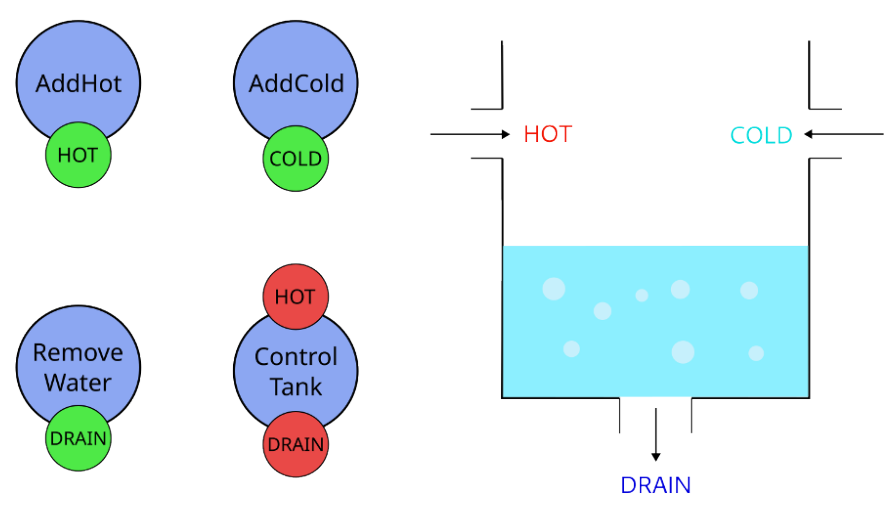
\includegraphics[width=\textwidth]{figures/bp-water-tank.png}
	\caption[Water Tank Example]{Water Tank Example; Water is too hot and too little, so \textit{HOT} and \textit{DRAIN} are blocked. Taken from \cite{felber_comprehensible_2025}.}
    \label{fig:bp-water-tank}
\end{figure}

During execution, the b-threads synchronize and vote on the next action.
An event is triggered only if it is requested and not vetoed by a supervising b-thread.
As shown in Figure~\ref{fig:bp-water-tank}, \textit{HOT} and \textit{DRAIN} are blocked in this depicted state because the water is too hot and the water level is too low.
This decoupled architecture allows developers to add new rules, such as a b-thread that prevents overflow, without altering the existing b-threads~\cite{harel_behavioral_2012}.